% !TeX encoding = UTF-8
% !TeX spellcheck = russian-aot
% !TeX program = pdflatex
\documentclass{beamer}

\usepackage[T1,T2A]{fontenc}
\usepackage[utf8]{inputenc}
\usepackage[russian]{babel}

\usepackage[linguistics]{forest}
\usepackage{booktabs}
\usepackage{pgfplots}
\usepackage{tikzducks}
\usepackage{comment}
\usepackage{listings}
\usepackage{amsmath}

\title{Алгоритмы параллельных вычислений. Сортировка слиянием (Algorithm M)}
\author{В.\,С.\,Верхотуров}
\institute{БСБО-05-20\\РТУ МИРЭА}
\date{\today}

\addtobeamertemplate{navigation symbols}{}{
	\usebeamerfont{footline}
	\usebeamercolor[fg]{footline}
	\hspace{1em}
	\insertframenumber/\inserttotalframenumber
}

\begin{document}
	
	\frame{\titlepage}
	
	\begin{frame}
		\frametitle{Содержание}
		
		\tableofcontents
	\end{frame}
	
	\section{Определение}
	
	\begin{comment}
		Сортировка слиянием --- это алгоритм «разделяй и властвуй». Он последовательно делит входной список длины n пополам, пока не останется n списков размера 1. Затем пары списков объединяются вместе с меньшим первым элементом среди пары списков, добавляемых на каждом шаге. Путем последовательного слияния и сравнения первых элементов строится отсортированный список.
	\end{comment}
	\begin{frame}
		\frametitle{Определение}
		Сортировка слиянием — это алгоритм <<разделяй и властвуй>>.
		
		\centering
		\begin{forest}
			[{[63, 74, 33, 50, 85, 62, 12]}
			[{[63, 74, 33]}
			[{[63]},name=head1]
			[,no edge[,no edge[,no edge[{[33, 63, 74]},no edge,name=foot2]]]]
			[{[74, 33]}
			[{[42]},name=head2d1]
			[,no edge[{[33, 74]},no edge,name=foot1]]
			[{[2]},name=head2d2]
			]
			]
			[,no edge[,no edge[,no edge[,no edge[,no edge[{[12, 33, 50, 62, 63, 74, 85]}, no edge, name=foot6]]]]]]
			[{[50, 85, 62, 12]}
			[{[50, 85]}
			[{[50]},name=head3d1]
			[,no edge[{[50, 85]},no edge,name=foot3]]
			[{[85]},name=head3d2]
			]
			[,no edge[,no edge[,no edge[{[12, 50, 62, 85]},no edge,name=foot5]]]]
			[{[62, 12]}
			[{[62]},name=head4d1]
			[,no edge[{[12, 62]},no edge,name=foot4]]
			[{[12]},name=head4d2]
			]
			]
			]
			\draw (head1) -- (foot2);
			\draw (head2d1) -- (foot1);
			\draw (head2d2) -- (foot1);
			\draw (head3d1) -- (foot3);
			\draw (head3d1) -- (foot3);
			\draw (head4d1) -- (foot4);
			\draw (head4d1) -- (foot4);
			\draw (head3d1) -- (foot3);
			\draw (foot1) -- (foot2);
			\draw (head3d2) -- (foot3);
			\draw (head4d2) -- (foot4);
			\draw (foot4) -- (foot5);
			\draw (foot3) -- (foot5);
			\draw (foot2) -- (foot6);
			\draw (foot5) -- (foot6);
		\end{forest}
	
	\end{frame}

	\begin{frame}
				\begin{equation}
			\phantom{00}\quad\phantom{00}\quad\phantom{00}\quad\phantom{00}\quad\left\{
			\begin{matrix}
				33 & 63 & 74 \\
				12 & 50 & 62 & 85
			\end{matrix}
			\right.
		\end{equation}
		
		\begin{equation}
			\phantom{00}\quad\phantom{00}\quad\phantom{00}\quad12\quad\left\{
			\begin{matrix}
				33 & 63 & 74 \\
				50 & 62 & 85 & \phantom{00}
			\end{matrix}
			\right.
		\end{equation}
		
		\begin{equation}
			\phantom{00}\quad\phantom{00}\quad12\quad33\quad\left\{
			\begin{matrix}
				63 & 74 \\
				50 & 62 & 85 & \phantom{00}
			\end{matrix}
			\right.
		\end{equation}
		
		\begin{equation}
			\phantom{00}\quad12\quad33\quad50\quad\left\{
			\begin{matrix}
				63 & 74 \\
				62 & 85 & \phantom{00} & \phantom{00}
			\end{matrix}
			\right.
		\end{equation}
		
		\begin{equation}
			12\quad33\quad50\quad62\quad\left\{
			\begin{matrix}
				63 & 74 \\
				85 & \phantom{00} & \phantom{00} & \phantom{00}
			\end{matrix}
			\right.
		\end{equation}
	\end{frame}

	\begin{frame}
		\begin{equation}
			\phantom{00}\quad\phantom{00}\quad12\quad33\quad50\quad62\quad63\quad\left\{
			\begin{matrix}
				74 \\
				85
			\end{matrix}
			\right.
		\end{equation}
	
		\begin{equation}
			\phantom{00}\quad12\quad33\quad50\quad62\quad63\quad74\quad\left\{
			\begin{matrix}
				\\
				85
			\end{matrix}
			\right.
		\end{equation}
	
		\begin{equation}
			12\quad33\quad50\quad62\quad63\quad74\quad85\quad\left\{
			\begin{matrix}
				\\
				\phantom{00}
			\end{matrix}
			\right.
		\end{equation}
	\end{frame}

	

	\section{Реализация сортировки в одном потоке}
	\begin{frame}[fragile]
		\frametitle{Реализация однопоточного алгоритма на CPython}
		
		\begin{lstlisting}[language=Python, basicstyle=\tiny]
from random import randint
from numbers import Number

def merge(arrays: list[list[Number]]) -> list[Number]:
	assert len(arrays) == 2
	x, y = arrays
	index_x = index_y = 0
	out = []
	while index_x < len(x) and \
			index_y < len(y):
		if x[index_x] < y[index_y]:
			out.append(x[index_x])
			index_x += 1
		else:
			out.append(y[index_y])
			index_y += 1
	out += x[index_x:] + y[index_y:]
	return out

def merge_sort(arr : list[Number]) -> list[Number]:
	if len(arr) <= 1:
		return arr
	if len(arr) == 2:
		return arr if arr[0] < arr[1] else [arr[1], arr[0]]
	mid = len(arr) // 2
	return merge(merge_sort(arr[:mid]), merge_sort(arr[mid:]))


def test_merge_sort():
	input_array = [randint(1, 100) for i in range(10)]
	print(merge_sort(input_array))

test_merge_sort()
		\end{lstlisting}
		
	\end{frame}

	\begin{frame}[fragile]
		\frametitle{Реализация однопоточного алгоритма на CPython. Часть~1}
		\begin{lstlisting}[language=Python]		
def test_merge_sort():
	input_array = [randint(1, 100) 
			for i in range(10)]
	print(merge_sort(input_array))

test_merge_sort()
		\end{lstlisting}
	
	\end{frame}

	\begin{frame}[fragile]
		\frametitle{Реализация однопоточного алгоритма на CPython. Часть~2}
		\begin{lstlisting}[language=Python]		
def merge_sort(arr : list[Number]) -> list[Number]:
	if len(arr) <= 1:
		return arr
	if len(arr) == 2:
		return arr 
			if arr[0] < arr[1] 
			else [arr[1], arr[0]]
	mid = len(arr) // 2
	return merge(merge_sort(arr[:mid]), 
		     merge_sort(arr[mid:]))
		\end{lstlisting}
	
	\end{frame}

	\begin{frame}[fragile]
		\frametitle{Реализация однопоточного алгоритма на CPython. Часть~3}
		\begin{lstlisting}[language=Python]		
def merge(arrays: list[list[Number]]) \
				-> list[Number]:
	assert len(arrays) == 2
	x, y = arrays
	index_x = index_y = 0
	out = []
	while index_x < len(x) and \
			index_y < len(y):
		if x[index_x] < y[index_y]:
			out.append(x[index_x])
			index_x += 1
		else:
			out.append(y[index_y])
			index_y += 1
	out += x[index_x:] + y[index_y:]
	return out
		\end{lstlisting}
	
	\end{frame}


	\section{Вычислительная и временная сложность}
	\begin{frame}
		\frametitle{Вычислительная сложность}
		
		Худшая выч. сложность:
		\begin{equation}
			O(n\log{}{n})
		\end{equation}
		
		Лучшая выч. сложность:
		\begin{equation}
			O(n\log{}{n})
		\end{equation}
		
		Средняя выч. сложность:
		\begin{equation}
			O(n\log{}{n})
		\end{equation}
	
		Временная сложность:
		\begin{multline}
			T^{sort}(n)=2T^{sort}\left(\frac{n}{2}\right)+T^{merge}(n)=\\=T^{sort}\left(\frac{n}{2}\right)+\Theta(\log^2{}{n})
		\end{multline}
	\end{frame}
	
	
	\begin{comment}
		merge exchange sort / сортировка Бетчера O( log(n)^2 )
		
		heapsort / пирамидальная сортировка O( n*log(n) )
	\end{comment}
	\begin{frame}
		
		\begin{tikzpicture}[scale=1.2]
			\begin{axis}[legend pos = south east, axis lines = left, grid = both, xlabel = $n$, ylabel = {$O(n)$}, ymax=100, xmax=100]
				\addplot [domain=0:100, samples=100, color=red]{x*log2(x)};
				\addlegendentry{$n\log{}{n}$};
				
				\addplot [domain=0:100, samples=100, color=green]{log2(x)^2};
				\addlegendentry{$\log^2{}{n}$};
				
				\addplot [domain=0:100, samples=100, color=blue]{x^2};
				\addlegendentry{$n^2$};
			\end{axis}
		\end{tikzpicture}
	\end{frame}


	\section{Параллельные вычисления в CPython}
	\begin{frame}[fragile]
		\frametitle{Параллельные вычисления в CPython (side-stepping the GIL (Global Interpreter Lock))}
		
		\begin{figure}
			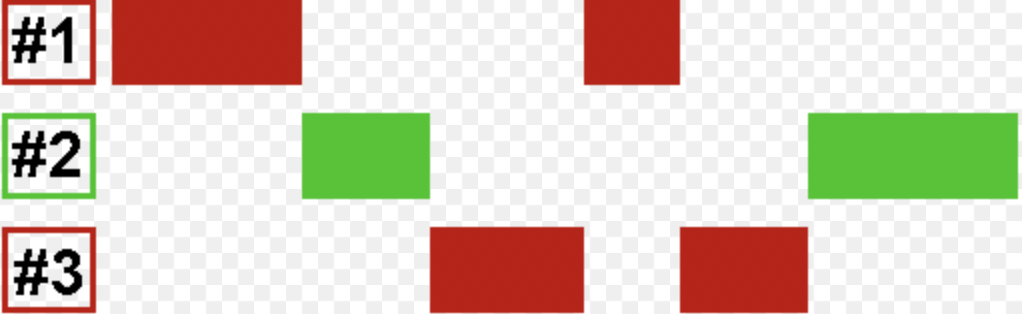
\includegraphics[width=5cm]{gil.png}
			\caption{Иллюстрация GIL}
		\end{figure}
		
		\begin{itemize}
			\item \verb*|multiprocessing.Process|, \verb*|multiprocessing.Pool| {\footnotesize\url{https://docs.python.org/3/library/multiprocessing.html}},
			\item C-расширение, расширение на Cython
			\item \verb*|os.system("python child.py")|, 
		\end{itemize}
		
		или...
		
	\end{frame}

	\section{Многопроцессная реализация алгоритма слияния}
	\begin{frame}[fragile]
		\frametitle{Многопроцессная реализация алгоритма слияния}
		
		\begin{lstlisting}[language=Python, basicstyle=\footnotesize]		
import multiprocessing
import math


def parallel_merge_sort(arr: list[Number]) -> list[Number]:
	processes = multiprocessing.cpu_count()
	pool = multiprocessing.Pool(processes = processes)
	size = math.ceil(len(arr) / processes)
	arr = [arr[i * size:(i + 1) * size] 
		for i in range(processes)]
	arr = pool.map(merge_sort, arr)
	while len(arr) > 1:
		extra = arr.pop() if len(arr) % 2 == 1 
				else None
		arr = [[arr[i], arr[i + 1]] 
			for i in range(0, len(arr), 2)]
		arr = pool.map(merge, arr) + \
			([extra] if extra else [])
	return arr[0]
		\end{lstlisting}
	\end{frame}

	
	\section{Временная сложность многопроцессного алгоритма}
	\begin{frame}
		\frametitle{Временная сложность}
		\begin{equation}
			T^{sort}(n)=T^{sort}\left(\frac{n}{2}\right)+T^{merge}(n)=T^{sort}\left(\frac{n}{2}\right)+\Theta(\log^2{}{n})
		\end{equation}
	\end{frame}


	\begin{frame}
		
		\centering
		\begin{tikzpicture}[scale=2.5]
			\duck[
			body=yellow!50!red!20!white,
			recedinghair=gray!50!white,
			eyebrow,
			tshirt=white!93!black,
			jacket=red!50!black,
			glasses=brown!70!lightgray,
			book=\scalebox{0.4}{\hspace{-2mm}\parbox{1.8cm}{The Art of Computer Programming. Volume~3. P.~158, 159}},
			bookcolour=black!20!brown
			]
		\end{tikzpicture}
		
		\vspace*{1cm}
		Код из презентации: \href{https://github.com/ValeryVerkhoturov/merge-sort-presentation}{github.com/ValeryVerkhoturov/merge-sort-presentation}
	
	\end{frame}

	
\end{document}